% PREAMBLE
\documentclass[11pt]{amsart}
\usepackage[T1]{fontenc}
\usepackage{lmodern}
\usepackage{microtype}
\usepackage{amsmath,amssymb}
\usepackage{mathtools}
\usepackage{graphicx}
\usepackage{booktabs}
\usepackage{tikz}
\usepackage[colorlinks=true,linkcolor=blue!45!black,citecolor=blue!45!black,urlcolor=blue!45!black]{hyperref}
\usepackage[capitalize]{cleveref}

\newtheorem{theorem}{Theorem}[section]
\newtheorem{proposition}[theorem]{Proposition}
\newtheorem{lemma}[theorem]{Lemma}
\newtheorem{corollary}[theorem]{Corollary}
\newtheorem{conjecture}[theorem]{Conjecture}
\theoremstyle{definition}
\newtheorem{definition}[theorem]{Definition}
\newtheorem{fact}[theorem]{Fact}
\theoremstyle{remark}
\newtheorem{remark}[theorem]{Remark}

\title[Base-3 Digit Designs]{Base-3 Digit Designs: Diagonality, Ray Masses, and a Spectral Gap at Two}
\author{Carlo Mitchener}
\email{carlo.mitchener@gmail.com}
\date{2026-08-23}

% PAPER
\begin{document}

\begin{abstract}
Draw a picture by writing numbers in base three and allowing only three of the nine possible digit pairs at each position; then ask which straight lines through the origin hit the picture, and how often. This paper answers three such questions for two families of base-three digit designs in the plane. First, a permutation design $F_\phi=\{(j,\phi(j))\}$ is \emph{diagonal}, meaning no two distinct points of any level share a ray through the origin, exactly when $\phi(0)\neq 0$; this holds for four of the six permutations of $\{0,1,2\}$, at every level, and is proved here. Second, for the Sierpi\'nski gasket design $G=\{(0,0),(1,0),(0,1)\}$ the number of points on a fixed ray obeys an exact linear recurrence: Fibonacci on $(3,1)$, Narayana's cows on $(1,12)$, and $c(m)=c(m-1)+c(m-4)$ on $(7,3)$, verified for all levels $n\le 30$. Third, for a coprime pair $(s,t)$ the growth rate of $\{z: z, sz, tz \in G_n\}$ is the spectral radius of an explicit carry automaton, trimmed to the states that can return to where they started, and over all $829$ coprime unordered pairs with $\max(s,t)\le 52$ that radius equals $3$ on the three shift pairs, equals $2$ on exactly twenty pairs, and never lands in the open interval $(2,3)$. Every number reported here is recomputed by a stdlib-only script that ships with the paper.
\end{abstract}

\maketitle

\section{Introduction}
\label{sec:intro}

\begin{figure}[!h]
\centering
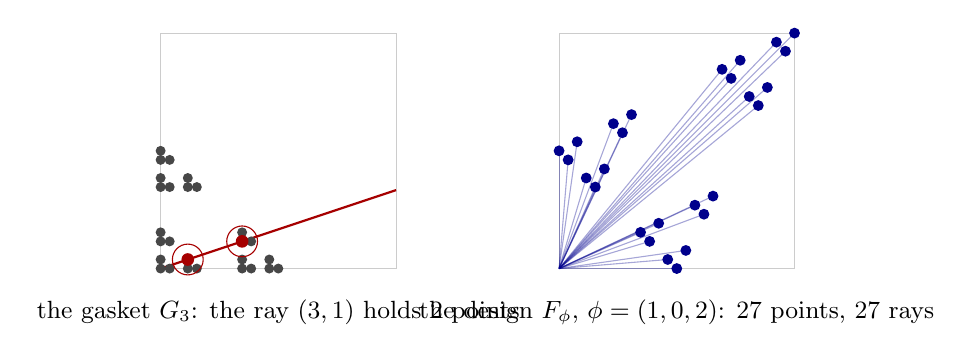
\begin{tikzpicture}[scale=0.115]
\begin{scope}
\draw[gray!40] (0,0) rectangle (26,26);
\draw[red!65!black, thick] (0,0) -- (26,8.667);
\foreach \a/\b in {0/0,0/1,0/3,0/4,0/9,0/10,0/12,0/13,1/0,1/3,1/9,1/12,3/0,3/9,3/10,4/0,4/9,9/0,9/1,9/4,10/0,10/3,12/0,12/1,13/0}
  \fill[black!72] (\a,\b) circle (0.55);
\foreach \a/\b in {3/1,9/3}
  {\fill[red!65!black] (\a,\b) circle (0.7); \draw[red!65!black] (\a,\b) circle (1.7);}
\node[below] at (13,-2.4) {\small the gasket $G_3$: the ray $(3,1)$ holds $2$ points};
\end{scope}
\begin{scope}[xshift=44cm]
\draw[gray!40] (0,0) rectangle (26,26);
\foreach \a/\b in {0/13,1/12,2/14,3/10,4/9,5/11,6/16,7/15,8/17,9/4,10/3,11/5,12/1,13/0,14/2,15/7,16/6,17/8,18/22,19/21,20/23,21/19,22/18,23/20,24/25,25/24,26/26}
  \draw[blue!55!black, opacity=0.35, line width=0.14mm] (0,0) -- (\a,\b);
\foreach \a/\b in {0/13,1/12,2/14,3/10,4/9,5/11,6/16,7/15,8/17,9/4,10/3,11/5,12/1,13/0,14/2,15/7,16/6,17/8,18/22,19/21,20/23,21/19,22/18,23/20,24/25,25/24,26/26}
  \fill[blue!55!black] (\a,\b) circle (0.6);
\node[below] at (13,-2.4) {\small the design $F_\phi$, $\phi=(1,0,2)$: $27$ points, $27$ rays};
\end{scope}
\end{tikzpicture}
\caption{Two base-3 digit designs at level $3$. On the left the gasket piles many points onto a few lines. On the right a diagonal design spreads every point onto a line of its own.}
\label{fig:rays}
\end{figure}

Write a nonnegative integer in base three. Now write two at once, stacked, so that position $i$ carries a pair of digits $(d^x_i, d^y_i)$ from the nine possibilities $\{0,1,2\}^2$. Choose three of those nine pairs and forbid the other six. The points you can still write form a self-similar cloud in the plane, and different choices of three give visibly different clouds. The question this paper asks is the simplest one available: which lines through the origin pass through the cloud, and how many of its points does each line catch? Two very different answers appear, depending on the design.

On the right of \cref{fig:rays} is a \emph{diagonal} design: no two of its $27$ points share a line through the origin, so the cloud meets $27$ distinct rays. This is not an accident of level three. \Cref{thm:diagonal} says that among the six designs of the form $F_\phi=\{(0,\phi(0)),(1,\phi(1)),(2,\phi(2))\}$, where $\phi$ permutes $\{0,1,2\}$, exactly four are diagonal at every level, and the test is as short as a test can be: $\phi(0)\neq 0$. The proof is elementary and complete. It rests on one observation, that every permutation of $\{0,1,2\}$ is an affine map $x\mapsto \alpha x+\beta$ over the field of three elements, and that after a cancellation the entire question collapses to whether $\beta=\phi(0)$ is zero.

On the left is the opposite extreme, the base-3 Sierpi\'nski gasket $G=\{(0,0),(1,0),(0,1)\}$. Here the points crowd onto lines, and the counting becomes interesting. Call $M_n(a,b)$ the number of nonzero level-$n$ gasket points on the ray through a primitive $(a,b)$. Then $M_n(3,1)$ runs $0$, $1$, $2$, $4$, $7$, $12$, $20$, $33$, one less than a Fibonacci number each time, and $M_n(1,12)$ runs $0$, $0$, $1$, $2$, $3$, $5$, $8$, $12$, $18$, one less than Narayana's cows \cite{oeisA000930}. These are exact identities for every level we have checked, not fits. The mechanism is not deep, and we say so plainly in \cref{sec:results}: an admissible digit string on a fixed ray is a word in a small carry automaton, and for these rays the automaton is a run-length constraint, so the counting sequences are the classical composition counts. What is new is the dictionary, not the arithmetic behind it.

The third question is about growth rather than counting. Fix coprime $(s,t)$ and ask how many gasket points $z$ have $sz$ and $tz$ also in the gasket. That set is again read by a carry automaton, and its growth rate is the spectral radius $\lambda(s,t)$ of the automaton once it is trimmed to the states that can get back to where they started (\cref{prop:growth}; the trimming is not optional, see \cref{rem:trim}). The answer has a hole in it. Over all $829$ coprime unordered pairs with $\max(s,t)\le 52$, the radius is $3$ on the three shift pairs $(1,3)$, $(1,9)$, $(1,27)$, is exactly $2$ on twenty further pairs, and otherwise sits at $1.6956\ldots$ or below. Nothing lands strictly between $2$ and $3$. The automaton is standard equipment; the hole is not.

The paper is short and self-contained. \Cref{sec:defs} fixes the objects. \Cref{sec:results} states the three laws, with tags: what is proved is labelled Theorem, Proposition, or Lemma and proved in \cref{sec:proofs}; what is checked over a stated finite range is labelled Fact, with that range written into the statement; what is believed is labelled Conjecture, with its evidence and the way it could fail. \Cref{sec:repro} names the script that recomputes every number.

\subsection*{Relation to existing work}

The tool is textbook. A set defined by a digit restriction in base $k$ is $k$-automatic, and reading it with a finite automaton whose states are carries is the standard method for such sets \cite{allouche}; the growth exponent of the accepted language is the Perron root of the transition matrix \cite{seneta}. The same device computes box dimensions of closed $k$-automatic sets, and base-$3$ multiplication automata are one of its stock examples \cite{kauto}. Nothing in \cref{sec:results} claims the machine as new. What the paper contributes is arithmetic output: an exact classification of the diagonal permutation designs, an exact dictionary between three gasket rays and three classical composition counts, and the observation that these particular automata have no Perron root in $(2,3)$, with an explicit largest value below $2$ and the pairs that attain it.

The mass laws deserve the same honesty. Narayana's cows counts compositions of $n$ into parts $1$ and $3$, and the Fibonacci numbers count binary strings with no two adjacent ones; the recurrence $c(m)=c(m-1)+c(m-4)$ counts compositions into parts $1$ and $4$. These are the most classical run-length counts there are. The content of \cref{fact:mass} is that particular gasket rays realise them, not that the sequences are surprising.

For the diagonality question we found no prior statement. The nearest literature is on radial projections and visible points of self-similar sets. A finite classification of the six base-$3$ permutation designs by a collinearity test is small enough that it is more likely unrecorded than known and forgotten; we state it, prove it, and make no priority claim.

\section{Definitions}
\label{sec:defs}

Throughout, $\mathbf{F}_3=\{0,1,2\}$ with arithmetic modulo $3$, and $n\ge 1$ is a level.

\begin{definition}[Digit design]
\label{def:design}
A \emph{digit design} is a three-element subset $F\subseteq\{0,1,2\}^2$. Its level-$n$ set is
\[
S_n(F)=\Bigl\{\textstyle\sum_{i=0}^{n-1} 3^i\, d_i \;:\; d_0,\dots,d_{n-1}\in F\Bigr\}\subseteq \mathbf{Z}^2 ,
\]
counted with the digit string that produces it, so that $S_n(F)$ carries $3^n$ strings. There are $\binom{9}{3}=84$ digit designs.
\end{definition}

Two families matter here, and they are different objects. Confusing them is the one trap in this subject.

\begin{definition}[The gasket, and the permutation designs]
\label{def:two}
The \emph{gasket design} is $G=\{(0,0),(1,0),(0,1)\}$, and we write $G_n=S_n(G)$; it is the base-$3$ Sierpi\'nski gasket truncated at level $n$. For a permutation $\phi$ of $\mathbf{F}_3$, the \emph{permutation design} is $F_\phi=\{(0,\phi(0)),(1,\phi(1)),(2,\phi(2))\}$. The gasket is not a permutation design and no permutation design is the gasket. \Cref{thm:diagonal} is about the $F_\phi$; \cref{fact:mass,fact:spectrum} are about $G$.
\end{definition}

\begin{definition}[Code of a design]
\label{def:code}
Index the nine cells by $3a+b$ for $(a,b)\in\{0,1,2\}^2$. The \emph{code} of a design is $\sum_{(a,b)\in F} 2^{3a+b}$. Under this indexing the four designs of \cref{thm:diagonal} have codes $98$ ($\phi=j+1$), $140$ ($\phi=j+2$), $266$ ($\phi$ swapping $0,1$) and $84$ ($\phi$ swapping $0,2$). The code $84$ is also what the transposed indexing $a+3b$ gives, so no convention rescues the value $148$, which names the cell set $\{(0,2),(1,1),(2,1)\}$ and is not a permutation design at all.
\end{definition}

\begin{definition}[Rays, mass, fibres]
\label{def:ray}
A \emph{primitive ray} is a pair $(a,b)$ of nonnegative integers, not both zero, with $\gcd(a,b)=1$; it stands for the half-line $\{z(a,b):z>0\}$. The two \emph{fibre rays} are $(1,0)$ and $(0,1)$. For a design $F$, the \emph{mass} of the ray $(a,b)$ at level $n$ is
\[
M_n^F(a,b)=\#\{z\ge 1 \;:\; z\,(a,b)\in S_n(F)\},
\]
and we drop the superscript when $F=G$. A ray is \emph{occupied} at level $n$ when its mass is positive. The origin lies on no ray.
\end{definition}

\begin{definition}[Diagonal design, and the count $Z_F$]
\label{def:diag}
A design $F$ is \emph{diagonal} when for every $n\ge 1$ no two distinct nonzero points of $S_n(F)$ are collinear with the origin, that is, when every occupied ray has mass $1$. Write $Z_F(n)$ for the number of occupied \emph{non-fibre} rays at level $n$.
\end{definition}

\begin{remark}[$Z$ is a ray count, not a second moment]
\label{rem:Z}
$Z_F(n)$ counts occupied non-fibre rays, each once. It is not the second moment $\sum_{(a,b)} M_n^F(a,b)^2$ over non-fibre rays. For a diagonal design the two agree, because every mass is $1$; for the gasket they differ wildly, and only the ray count is meant anywhere in this paper.
\end{remark}

\begin{definition}[Multiplier-pair automaton]
\label{def:auto}
Fix coprime integers $1\le s<t$. The automaton $\mathcal{A}(s,t)$ has states in $\mathbf{Z}^2\times\mathbf{Z}^2$, start state $(0,0;0,0)$, and from a state $(\mathbf{a};\mathbf{b})$ a digit $d\in G$ is admissible when
\[
(s\,d+\mathbf{a}) \bmod 3 \in G \quad\text{and}\quad (t\,d+\mathbf{b}) \bmod 3 \in G ,
\]
with the reductions taken componentwise; the successor state is then $\bigl(\lfloor (s\,d+\mathbf{a})/3\rfloor;\lfloor (t\,d+\mathbf{b})/3\rfloor\bigr)$, again componentwise. Reading the base-$3$ digits of $z$ from least significant, a path of length $n$ from the start state that returns to the start state records exactly a $z$ with $z, sz, tz\in G_n$. Call a state \emph{live} when it is both reachable from the start state and able to reach the start state; only live states lie on such a path, and there are finitely many of them. Write $T(s,t)$ for the transition matrix carried by the live states, and $\lambda(s,t)$ for its spectral radius. The pair $(s,t)$ is a \emph{shift pair} when $\{s,t\}=\{1,3^j\}$ for some $j\ge 1$, the case in which multiplication is a digit shift.
\end{definition}

\begin{remark}[Trimming to the live states is not cosmetic]
\label{rem:trim}
Take $(s,t)=(1,16)$. The automaton reaches eleven states, but only the start state is live: every other reachable state leads away and never comes back. So $T(1,16)$ is the $1\times 1$ matrix $(1)$, carrying the loop on the digit $(0,0)$, and $\lambda(1,16)=1$. By \cref{prop:growth} this says $\#\{z: z, 16z\in G_n\}=1$ for every $n$, that is, only $z=0$ qualifies, which is correct. Had we taken the spectral radius of the whole reachable set we would have got the plastic number $1.3247\ldots$, which measures how fast admissible digit strings accumulate, not how many of them close up into a point. Thirteen of the $829$ pairs of \cref{fact:spectrum} are affected by the trimming, and all thirteen drop to $\lambda=1$.
\end{remark}

\section{Results}
\label{sec:results}

\subsection{Law 1: which permutation designs are diagonal}

\begin{lemma}[Cross lemma]
\label{lem:cross}
Let $\phi$ be a permutation of $\mathbf{F}_3$ and let $x,x'\in S_n(F_\phi)$ come from distinct digit strings $d\neq d'$, first differing at position $k$. Then
\[
\det(x,x') \;=\; x_1x_2'-x_2x_1' \;\equiv\; 3^k\,\phi(0)\,(d_k-d_k') \pmod{3^{k+1}} .
\]
In particular, if $\phi(0)\neq 0$ then $v_3(\det(x,x'))=k$ exactly, so $\det(x,x')\neq 0$.
\end{lemma}

\begin{theorem}[Diagonal classification]
\label{thm:diagonal}
Let $\phi$ be a permutation of $\mathbf{F}_3$. Then $F_\phi$ is a diagonal design if and only if $\phi(0)\neq 0$. Four of the six permutations qualify: $j\mapsto j+1$, $j\mapsto j+2$, the swap of $0$ and $1$, and the swap of $0$ and $2$. For each of these four and every $n\ge 1$, the $3^n$ level-$n$ digit strings give $3^n$ distinct nonzero points on $3^n$ distinct rays, exactly two of which are fibre rays, so
\[
Z_{F_\phi}(n)=3^n-2 \qquad (n\ge 1).
\]
For the two permutations with $\phi(0)=0$ the design is not diagonal: the identity fails at level $1$, where $(1,1)$ and $(2,2)$ share a ray, and $\phi(j)=2j$ fails at level $2$, where $(1,2)$ and $(3,6)$ share a ray.
\end{theorem}

\begin{remark}[The bound starts at $n=1$]
\label{rem:n1}
The formula $Z_{F_\phi}(n)=3^n-2$ is false at $n=0$: the empty digit string gives the origin, which lies on no ray, so $Z_{F_\phi}(0)=0$ while $3^0-2=-1$. The statement is scoped to $n\ge 1$ throughout.
\end{remark}

Diagonality by itself, without the permutation hypothesis, is a slightly weaker condition, and the following census says exactly how much weaker.

\begin{fact}[Census of the 84 designs]
\label{fact:census84}
Among the $84$ digit designs, exactly $10$ have the property that for every level $n\le 6$ no two distinct nonzero points of $S_n(F)$ are collinear with the origin. Exactly $4$ of those $10$ are permutation designs, namely the four of \cref{thm:diagonal}. The other six are
\[
\begin{array}{lll}
\{(0,1),(1,1),(2,1)\}, & \{(0,2),(1,2),(2,2)\}, & \{(1,0),(1,1),(1,2)\},\\
\{(1,1),(1,2),(2,1)\}, & \{(1,2),(2,1),(2,2)\}, & \{(2,0),(2,1),(2,2)\};
\end{array}
\]
they are not permutation designs, and while four of them do have a constant coordinate, the two designs $\{(1,1),(1,2),(2,1)\}$ and $\{(1,2),(2,1),(2,2)\}$ do not. The four permutation designs are also exactly the survivors that occupy two fibre rays; the other six occupy one or none. Hence the sharp criterion inside the census is ``no two points collinear, and exactly two fibre rays occupied''. Checked by \texttt{scripts/verify.py} over all $84$ designs and levels $1\le n\le 6$.
\end{fact}

\subsection{Law 2: how much mass each gasket ray carries}

The gasket is the opposite of diagonal, so masses are the interesting invariant. One global count is immediate and exact at every level.

\begin{proposition}[Total non-fibre mass]
\label{prop:total}
For every $n\ge 0$, the number of nonzero level-$n$ gasket points lying off both fibre rays is
\[
\sum_{(a,b)\ \mathrm{non\text{-}fibre}} M_n(a,b) \;=\; 3^n-2^{n+1}+1 .
\]
At $n=12$ this is $531441-8192+1=523250$.
\end{proposition}

\begin{fact}[Ray mass laws]
\label{fact:mass}
Let $F(1)=F(2)=1$ be the Fibonacci numbers \cite{oeisA000045}, let $a(0)=a(1)=a(2)=1$ and $a(m)=a(m-1)+a(m-3)$ be Narayana's cows \cite{oeisA000930}, and let $c(0),c(1),c(2),c(3)=1,2,3,4$ with $c(m)=c(m-1)+c(m-4)$ for $m\ge 4$. Then for every level $n$ in the stated range:
\begin{enumerate}
\item $M_n(3,1)=F(n+1)-1$ for $1\le n\le 30$;
\item $M_n(3^j,1)=\bigl(\prod_{r=0}^{j-1} F(m_r+2)\bigr)-1$ for $1\le j\le 13$ and $1\le n\le 30$, where $m_r=\#\{i\in[0,n-j): i\equiv r \bmod j\}$;
\item $M_n(1,12)=a(n)-1$ for $1\le n\le 30$;
\item $M_n(7,3)=c(n-3)-1$ for $3\le n\le 30$.
\end{enumerate}
Checked by \texttt{scripts/verify.py}, which builds a bounded-carry automaton for each ray and cross-checks it against enumeration of the gasket points themselves: directly over all $3^n$ points for $1\le n\le 10$, and for $1\le n\le 14$ by splitting each point as $u+3^{\lfloor n/2\rfloor}v$ with $u,v$ in gasket sets of half the level, which counts the same $3^n$ points without listing them.
\end{fact}

\begin{remark}[The seeds are $1,2,3,4$, not $1,1,1,1$]
\label{rem:seeds}
The $(7,3)$ recurrence must be started at $c(0),c(1),c(2),c(3)=1,2,3,4$. Starting it at $1,1,1,1$ produces a different sequence and the identity in \cref{fact:mass}(4) fails immediately.
\end{remark}

\begin{remark}[Squares on the ray $(7,3)$]
\label{rem:squares}
$M_{14}(7,3)=49=7^2$ is not singular. The mass is a perfect square at exactly $n=4,7,9,12,14$ in the range $1\le n\le 30$, with values $1,4,9,25,49$, and at no $n$ in $15\le n\le 30$. There is also no algebraic reason to expect squares: the characteristic polynomial $x^4-x^3-1$ of the recurrence is irreducible over $\mathbf{Q}$. Indeed it has no rational root, since by the rational root theorem the only candidates are $\pm 1$ and neither is a root; and by Gauss's lemma a factorisation into two rational quadratics may be taken integral, $(x^2+ax+b)(x^2+cx+d)$, which forces $bd=-1$, so $\{b,d\}=\{1,-1\}$ and the linear coefficient $ad+bc=\pm(a-c)$ vanishes only if $a=c$, contradicting $a+c=-1$ in the integers.
\end{remark}

\begin{fact}[The level-12 census]
\label{fact:census12}
At level $n=12$ the gasket has $3^{12}=531441$ points. Exactly $345318$ non-fibre primitive rays are occupied, and they carry $523250$ points in total, in agreement with \cref{prop:total}. Ray mass is symmetric under $x\leftrightarrow y$, so occupied rays come in equal-mass mirror pairs; the ten heaviest are five shift rays and their five mirrors:
\begin{center}
\begin{tabular}{lrrrrr}
\toprule
ray & $(3,1)$ & $(9,1)$ & $(27,1)$ & $(81,1)$ & $(243,1)$ \\
\midrule
mass & $232$ & $168$ & $124$ & $80$ & $71$ \\
\bottomrule
\end{tabular}
\end{center}
and $232=F(13)-1$. Checked by \texttt{scripts/verify.py} by literal enumeration of all $531441$ points, with the total mass identity of \cref{prop:total} rechecked at every level $1\le n\le 12$.
\end{fact}

\subsection{Law 3: how fast a pair of multiples can grow}

\begin{proposition}[The radius is the growth rate]
\label{prop:growth}
Let $1\le s<t$ be coprime and let $T=T(s,t)$ be the live transition matrix of \cref{def:auto}, with the start state carrying index $0$. Then for every $n\ge 0$
\[
\#\{z : z, sz, tz\in G_n\}=(T^n)_{00} ,
\]
and consequently
\[
\lim_{n\to\infty}\ \#\{z : z, sz, tz\in G_n\}^{1/n}=\lambda(s,t).
\]
\end{proposition}

\begin{fact}[Spectral gap at two]
\label{fact:spectrum}
Let $(s,t)$ range over the $829$ coprime unordered pairs with $1\le s<t\le 52$. Then:
\begin{enumerate}
\item $\lambda(s,t)=3$ for exactly three pairs, namely the shift pairs $(1,3)$, $(1,9)$, $(1,27)$;
\item no pair has $\lambda(s,t)$ in the open interval $(2,3)$;
\item $\lambda(s,t)=2$ for exactly twenty pairs, listed in \cref{tab:two};
\item the largest value strictly below $2$ is $\lambda=1.6956207695598\ldots$, attained by $25$ pairs, the smallest being $(1,13)$ and including $(12,13)$; the next value down is $1.6769719158912\ldots$, attained by $(1,31)$, $(3,31)$, $(9,31)$ and $(27,31)$;
\item the pairs $(2,9)$ and $(1,18)$, whose multipliers are divisible by $9$ after reordering, have $\lambda=1$: their live sets are the start state alone.
\end{enumerate}
Checked by \texttt{scripts/verify.py}, which builds each automaton from \cref{def:auto}, trims it to its live states, forms the characteristic polynomial by Faddeev--LeVerrier in exact integer arithmetic, and certifies the absence of a real root above a rational $r$ by shifting the polynomial to $r$ and observing that every coefficient is nonnegative. Because the transition matrix is nonnegative, its spectral radius is itself a real eigenvalue, so this certificate is a proof of $\lambda\le r$ for each individual pair. Every quoted decimal is pinned from both sides in exact rational arithmetic: the upper side by that certificate, the lower side by a rational point at which the characteristic polynomial is negative, which forces a real root above it.
\end{fact}

\begin{table}[ht]
\centering
\begin{tabular}{llllll}
\toprule
$(1,4)$ & $(1,7)$ & $(1,10)$ & $(1,12)$ & $(1,21)$ & $(1,28)$ \\
$(1,30)$ & $(1,36)$ & $(3,4)$ & $(3,7)$ & $(3,10)$ & $(3,28)$ \\
$(4,9)$ & $(4,27)$ & $(7,9)$ & $(7,27)$ & $(9,10)$ & $(9,28)$ \\
$(10,27)$ & $(27,28)$ & & & & \\
\bottomrule
\end{tabular}
\caption{The twenty coprime pairs with $\max(s,t)\le 52$ attaining $\lambda=2$ exactly.}
\label{tab:two}
\end{table}

The simplest attainer can be checked by hand, so we prove it.

\begin{proposition}[The pair $(1,4)$]
\label{prop:one4}
The automaton $\mathcal{A}(1,4)$ has exactly three reachable states, all of them live: $A=(0,0;0,0)$, $B=(0,0;1,0)$ and $C=(0,0;0,1)$, with transitions $A\to A$, $A\to B$, $A\to C$, $B\to A$, $C\to A$. Its characteristic polynomial is $\lambda^3-\lambda^2-2\lambda=\lambda(\lambda-2)(\lambda+1)$, so $\lambda(1,4)=2$. The number $G_m$ of paths of length $m$ that start at $A$, ending anywhere, satisfies
\[
G_m=G_{m-1}+2G_{m-2}\quad (m\ge 2), \qquad G_0=1,\ G_1=3,
\]
whence $G_m=\bigl(2^{m+2}-(-1)^m\bigr)/3$, giving $1$, $3$, $5$, $11$, $21$, $43$, $85$, $171$, and $G_{15}=43691$. The arithmetic count is the number $R_m=(T^m)_{AA}$ of paths that return to $A$, which obeys the same recurrence from $R_0=R_1=1$, so
\[
\#\{z: z, 4z\in G_m\}=R_m=\bigl(2^{m+1}+(-1)^m\bigr)/3 ,
\]
giving $1$, $1$, $3$, $5$, $11$, $21$, $43$, $85$, $171$, and $R_{15}=21845$. Both grow like $2^m$, but only $R_m$ counts points.
\end{proposition}

\subsection{What is not proved}

\begin{conjecture}[The mass laws hold at every level]
\label{con:mass}
The four identities of \cref{fact:mass} hold for every $n$, not only for $n\le 30$.
\smallskip

\noindent\emph{Evidence.} Each identity is an equality of two linear recurrences with the same order; agreement over $30$ consecutive levels is far more than the order of either recurrence. The counting side is generated by a finite bounded-carry automaton, which strongly suggests eventual linearity. Two independent implementations agree, and enumeration of the gasket points themselves, split into halves as in \cref{fact:mass}, agrees for $n\le 14$.
\smallskip

\noindent\emph{Failure mode.} A carry state reachable only at large $n$ would add a term to the recurrence and break the identity at a level beyond the checked range. This is exactly what a written bijection between admissible digit strings and compositions would rule out; no such bijection is written here, and until one is, the identities are checked, not proved.
\end{conjecture}

\begin{conjecture}[The gap is universal]
\label{con:gap}
For every coprime pair $(s,t)$ with $s<t$, $\lambda(s,t)\in\{3\}\cup[0,2]$; that is, the open interval $(2,3)$ contains no Perron root of any $\mathcal{A}(s,t)$, and $\lambda(s,t)=3$ only for shift pairs.
\smallskip

\noindent\emph{Evidence.} All $829$ coprime pairs with $\max(s,t)\le 52$ obey it, each certified by exact integer arithmetic rather than by a numerical eigenvalue. The values cluster: $3$, then $2$, then $1.6956\ldots$ and below, with a clean gap of width $0.30\ldots$ under $2$ as well as the full width of $(2,3)$ above it. The state counts stay small, at most $45$ reachable and at most $33$ live over the whole range, so the automata do not appear to be growing in a way that would eventually fill the interval.
\smallskip

\noindent\emph{Failure mode.} A pair with a large multiplier could have a much larger reachable state set and a Perron root anywhere in $(2,3)$; nothing in the finite check bounds the state count for general $(s,t)$. A proof would need a uniform argument, for instance a subinvariant vector $v>0$ with $\mathcal{A}v\le 2v$ constructed for every non-shift pair at once.
\end{conjecture}

\begin{remark}[Open direction]
\label{rem:open}
\Cref{fact:spectrum} bounds pairs, not triples or larger families, and a bound on pairs alone gives only a crude bound on the number of occupied gasket rays. Extending the gap from pairs to $k$-tuples of multipliers is the natural next question and is not addressed here.
\end{remark}

\section{Proofs}
\label{sec:proofs}

\begin{proof}[Proof of \cref{lem:cross}]
Write $x=\sum_{i<n} 3^i (d_i,\phi(d_i))$, and likewise for $x'$ with digits $d_j'$. Bilinearity gives
\[
\det(x,x')=\sum_{i,j<n} 3^{i+j}\, w(d_i,d_j'), \qquad w(u,v):=u\,\phi(v)-\phi(u)\,v .
\]
The form $w$ is antisymmetric, $w(v,u)=-w(u,v)$, and $w(u,u)=0$.

Collect the coefficient of $3^m$:
\[
C_m=\sum_{\substack{i+j=m\\ 0\le i,j<n}} w(d_i,d_j') .
\]
Fix $m<k$. Every index occurring in $C_m$ is at most $m<k$, and $d$ and $d'$ agree below $k$, so $d_j'=d_j$ for all such $j$ and $C_m=\sum_{i+j=m} w(d_i,d_j)$. Pair the term $(i,j)$ with the term $(j,i)$: the two cancel by antisymmetry, and a term with $i=j$ vanishes on its own. Hence $C_m=0$ for every $m<k$, and $v_3(\det(x,x'))\ge k$.

Now take $m=k$. The terms are indexed by $i=0,\dots,k$ with $j=k-i$. For $1\le i\le k-1$ both indices are strictly below $k$, so as above those terms cancel in pairs and contribute nothing. What remains is $i\in\{0,k\}$:
\[
C_k=w(d_0,d_k')+w(d_k,d_0') .
\]
If $k=0$ the two displayed terms are the single term $w(d_0,d_0')$, and the computation below still applies verbatim. If $k\ge 1$ then $d_0'=d_0$, so, using antisymmetry,
\[
C_k=w(d_0,d_k')-w(d_0,d_k)=\phi(d_0)\bigl(d_k-d_k'\bigr)-d_0\bigl(\phi(d_k)-\phi(d_k')\bigr).
\]

It remains to evaluate $C_k$ modulo $3$. Every permutation of $\mathbf{F}_3$ is affine: the affine maps $x\mapsto \alpha x+\beta$ with $\alpha\in\{1,2\}$ and $\beta\in\{0,1,2\}$ are six distinct permutations, and $\mathbf{F}_3$ has only six permutations, so they are all of them. Writing $\phi(x)=\alpha x+\beta$ and noting $\beta=\phi(0)$,
\begin{align*}
C_k &\equiv (\alpha d_0+\beta)(d_k-d_k')-d_0\,\alpha\,(d_k-d_k')\\
&= \beta\,(d_k-d_k') \equiv \phi(0)\,(d_k-d_k') \pmod 3 .
\end{align*}
This is the stated congruence. If $\phi(0)\neq 0$ then both factors of $\phi(0)(d_k-d_k')$ are nonzero in the field $\mathbf{F}_3$, because $d_k\neq d_k'$, so $C_k\not\equiv 0 \pmod 3$ and $v_3(\det(x,x'))=k$ exactly. A number of finite $3$-adic valuation is nonzero.
\end{proof}

\begin{proof}[Proof of \cref{thm:diagonal}]
Suppose $\phi(0)\neq 0$. Then no digit of $F_\phi$ is $(0,0)$, so no level-$n$ point is the origin for $n\ge 1$. Distinct digit strings give distinct points, because the first coordinate $\sum_i d_i 3^i$ with $d_i\in\{0,1,2\}$ is a base-$3$ representation and so recovers the string. By \cref{lem:cross}, for any two distinct digit strings the cross determinant is nonzero, so the two points are not collinear with the origin. Hence the $3^n$ points sit on $3^n$ distinct rays, every occupied ray has mass $1$, and $F_\phi$ is diagonal.

Count the fibre rays. A level-$n$ point has second coordinate $0$ exactly when $\phi(d_i)=0$ for every $i$, that is, when every digit equals $c:=\phi^{-1}(0)$; since $\phi(0)\neq 0$ we have $c\neq 0$, and the single string $d_i=c$ for all $i$ gives one point, which is nonzero because its first coordinate is $c(3^n-1)/2>0$. So the fibre ray $(1,0)$ is occupied, by exactly one point. Symmetrically the first coordinate vanishes exactly when every digit is $0$, giving the single point $\bigl(0,\phi(0)(3^n-1)/2\bigr)$, so the fibre ray $(0,1)$ is occupied by exactly one point. No point lies on both, since it would be the origin. Therefore exactly two of the $3^n$ occupied rays are fibre rays and
\[
Z_{F_\phi}(n)=3^n-2 \qquad (n\ge 1),
\]
which is the claim.

Conversely suppose $\phi(0)=0$. There are two such permutations. For the identity, $F_{\mathrm{id}}=\{(0,0),(1,1),(2,2)\}$ and at level $1$ the points $(1,1)$ and $(2,2)$ satisfy $1\cdot 2-1\cdot 2=0$, so they are collinear with the origin and $F_{\mathrm{id}}$ is not diagonal. For $\phi(j)=2j$, that is $F_\phi=\{(0,0),(1,2),(2,1)\}$, level $1$ is fine but level $2$ is not: the digit string $(d_0,d_1)=(1,0)$ gives $(1,2)$ and the string $(0,1)$ gives $(3,6)$, and $1\cdot 6-2\cdot 3=0$. So $F_\phi$ is not diagonal either. This proves the equivalence, and the four qualifying permutations are exactly those with $\beta=\phi(0)\neq 0$, namely $x\mapsto x+1$, $x\mapsto x+2$, $x\mapsto 2x+1$ (the swap of $0$ and $1$) and $x\mapsto 2x+2$ (the swap of $0$ and $2$).
\end{proof}

\begin{proof}[Proof of \cref{prop:total}]
The level-$n$ gasket has $3^n$ points, one per digit string, and distinct strings give distinct points because the pair of coordinates determines each digit. A point lies on the fibre ray $(1,0)$ or is the origin exactly when its second coordinate vanishes, that is when every digit lies in $\{(0,0),(1,0)\}$: that is $2^n$ strings. Symmetrically $2^n$ strings give second-coordinate points with first coordinate $0$. The two families meet in the single all-$(0,0)$ string, the origin. So the number of points that are nonzero and off both fibres is
\[
3^n-\bigl(2^n+2^n-1\bigr)=3^n-2^{n+1}+1 ,
\]
and this count is precisely the sum of the masses of the non-fibre rays, since every such point lies on exactly one primitive ray.
\end{proof}

\begin{proof}[Proof of \cref{prop:growth}]
A point $z\in G_n$ is the same thing as a digit string $d_0,\dots,d_{n-1}\in G$, and distinct strings give distinct points. Run $\mathcal{A}(s,t)$ on that string. By construction the state after $i$ steps is the pair of carries left by multiplying $z$ by $s$ and by $t$, and the digit $d_i$ is admissible exactly when the base-$3$ digit at position $i$ of $sz$ and of $tz$ both lie in $G$. If the path is back at the start state after $n$ steps then both carries vanish, so $sz$ and $tz$ have all digits in $G$ and nothing above position $n-1$, that is $sz,tz\in G_n$; conversely if $sz,tz\in G_n$ then every step is admissible and the carries after $n$ steps are zero, so the path returns. Closed paths of length $n$ at the start state are therefore in bijection with the points counted. No closed path through the start state visits a state that is not live, so the count is unchanged by the trimming and equals $(T^n)_{00}$.

Every live state lies on a closed path through the start state, hence is in the same strongly connected component as the start state, so the live digraph is strongly connected. The digit $(0,0)$ is admissible at the start state and returns to it, so the digraph carries a loop. A nonnegative matrix whose digraph is strongly connected and carries a loop is primitive, and for a primitive matrix $T^n=\lambda^n(vw^{\mathsf T}+o(1))$ with $v,w>0$, so $(T^n)_{00}^{1/n}\to\lambda$ \cite[Ch.~1]{seneta}.
\end{proof}

\begin{proof}[Proof of \cref{prop:one4}]
Take $s=1$, $t=4$ in \cref{def:auto}. From the start state $A=(0,0;0,0)$ the digit $(0,0)$ produces output digits $(0,0)$ and $(0,0)$ with no carry, returning to $A$; the digit $(1,0)$ produces $1\cdot(1,0)=(1,0)$, admissible with no carry, and $4\cdot(1,0)=(4,0)\equiv (1,0) \bmod 3$ with carry $(1,0)$, so the successor is $B=(0,0;1,0)$; symmetrically the digit $(0,1)$ leads to $C=(0,0;0,1)$. From $B$, the digit $(0,0)$ gives second-track value $(1,0)$, admissible, with successor carry $(0,0)$, so $B\to A$; the digits $(1,0)$ and $(0,1)$ give second-track values $(5,0)\equiv (2,0)$ and $(1,1)$ respectively, neither in $G$, so they are inadmissible. Symmetrically $C\to A$ only. No further states are reachable, so the reachable set is $\{A,B,C\}$ with the transition matrix
\[
T=\begin{pmatrix} 1&1&1\\ 1&0&0\\ 1&0&0\end{pmatrix}.
\]
Its trace is $1$, the sum of its principal $2\times 2$ minors is $(-1)+(-1)+0=-2$, and its determinant is $0$ because the last two rows agree; hence $\det(\lambda I-T)=\lambda^3-\lambda^2-2\lambda=\lambda(\lambda-2)(\lambda+1)$ and the spectral radius is $2$.

For the count, let $G_m$ be the number of paths of length $m$ starting at $A$. Such a path either begins with the loop $A\to A$, leaving a path of length $m-1$ from $A$, or begins with $A\to B$ or $A\to C$, in which case the next step is forced back to $A$ and leaves a path of length $m-2$ from $A$. Hence $G_m=G_{m-1}+2G_{m-2}$ for $m\ge 2$, with $G_0=1$ and $G_1=3$. Solving the recurrence with roots $2$ and $-1$ gives $G_m=\bigl(2^{m+2}-(-1)^m\bigr)/3$, and $G_{15}=(2^{17}+1)/3=43691$. The same split applies to paths that return to $A$, since after $A\to B\to A$ or $A\to C\to A$ the walk is again at $A$: writing $R_m$ for their number, $R_m=R_{m-1}+2R_{m-2}$ for $m\ge 2$ with $R_0=R_1=1$, so $R_m=\bigl(2^{m+1}+(-1)^m\bigr)/3$ and $R_{15}=(2^{16}-1)/3=21845$. By \cref{prop:growth} it is $R_m$, not $G_m$, that counts the $z$ with $z,4z\in G_m$.
\end{proof}

\section{Reproducibility}
\label{sec:repro}

Two scripts ship with the paper. Both are plain \texttt{python3} with no dependencies outside the standard library, take no arguments, read nothing, and use only relative paths. Run them from the paper's directory.

\texttt{python3 scripts/verify.py} runs in about two seconds and recomputes every number in \cref{sec:results}. It covers, in order:
\begin{itemize}
\item all $84$ digit designs at levels $1\le n\le 6$, confirming the ten survivors and the four permutation designs of \cref{fact:census84}, their codes $84,98,140,266$ under the indexing of \cref{def:code}, the fibre counts, and that the cell set named by $148$ is not a permutation design;
\item the cross coefficient of \cref{lem:cross} in all $18$ cases $(d_0,d_k,d_k')$ for each of the six permutations, confirming both that it is nonzero exactly when $\phi(0)\neq 0$ and that it equals $\phi(0)(d_k-d_k')$ modulo $3$;
\item $Z_{F_\phi}(n)=3^n-2$ for the four diagonal designs and $1\le n\le 8$, $Z_{F_\phi}(0)=0$, and the two explicit collinear witnesses of \cref{thm:diagonal};
\item \cref{fact:mass}: rays $(3,1)$, $(1,12)$ and $(7,3)$ for $n\le 30$, the thirteen shift rays $(3^j,1)$ for $1\le j\le 13$ and $n\le 30$ against the Fibonacci product, and the bounded-carry automaton against direct enumeration of all $3^n$ points for six rays and $1\le n\le 10$, and against the split enumeration for the same six rays and $1\le n\le 14$;
\item the perfect-square levels of \cref{rem:squares} over $1\le n\le 30$, and the two cases that make $x^4-x^3-1$ irreducible;
\item \cref{prop:total} at every level $1\le n\le 12$, and \cref{fact:census12} by enumerating all $531441$ level-$12$ points, including the ten heaviest rays and the mirror symmetry;
\item \cref{fact:spectrum}: all $829$ coprime unordered pairs with $\max(s,t)\le 52$, each trimmed to its live states and given an exact integer characteristic polynomial with a nonnegative-shift certificate, plus a bisection in exact rational arithmetic and two-sided rational windows pinning $1.6956207695598\ldots$ with its $25$ attainers and $1.6769719158912\ldots$ with its four, the largest reachable and live state counts $45$ and $33$, the trimming trap of \cref{rem:trim} at $(1,16)$, the return counts of \cref{prop:growth} against direct enumeration for $n\le 8$, and the explicit data of \cref{prop:one4} including the recurrence residuals through $m=15$.
\end{itemize}
Every assertion names the quantity, the value obtained, and the value expected, and the script stops at the first mismatch. A successful run ends with \texttt{all green} and exit status $0$.

\texttt{python3 scripts/figure.py} runs in well under a second and writes \texttt{figures/rays.svg}, the two-panel picture used outside the paper; the version inside the paper, \cref{fig:rays}, is drawn in \TeX.

\texttt{tectonic paper.tex} rebuilds \texttt{paper.pdf}.

\section*{Acknowledgments}

This paper was developed and verified in collaboration with Claude (Anthropic). The author takes sole responsibility for every claim.

\begin{thebibliography}{9}

\bibitem{allouche}
J.-P. Allouche and J. Shallit, \emph{Automatic Sequences: Theory, Applications,
Generalizations}, Cambridge University Press, 2003. \url{https://doi.org/10.1017/CBO9780511546563}

\bibitem{kauto}
A. Block Gorman and C. Schulz, \emph{Fractal dimensions of $k$-automatic sets}, preprint, 2022. arXiv:2205.02915. \url{https://arxiv.org/abs/2205.02915}

\bibitem{oeisA000045}
OEIS Foundation Inc., \emph{Sequence A000045 (Fibonacci numbers)}, The On-Line Encyclopedia of Integer Sequences. \href{https://oeis.org/A000045}{https://oeis.org/A000045}

\bibitem{oeisA000930}
OEIS Foundation Inc., \emph{Sequence A000930 (Narayana's cows sequence)}, The On-Line Encyclopedia of Integer Sequences. \href{https://oeis.org/A000930}{https://oeis.org/A000930}

\bibitem{seneta}
E. Seneta, \emph{Non-negative Matrices and Markov Chains}, 2nd ed., Springer, 1981. \url{https://doi.org/10.1007/0-387-32792-4}

\end{thebibliography}

\end{document}
